
\documentclass{article}

\usepackage{amssymb}
\usepackage{mathrsfs}
\usepackage{graphicx}

\setlength\parindent{0pt} % Removes all indentation from paragraphs
\renewcommand\footnoterule{\rule{\linewidth}{0.4pt}}

\begin{document}
\title{Physics Problems:\\ Problem \#2}

\author{For Lucas}

\date{\today}
\maketitle


\section*{The Ferret\footnote{Gn\"adig, Honyek \& Riley. \textit{200 Puzzling Physics Problems}. Problem 13. }}

A small ferret is put into a circular wheel-cage, which has a frictionless central pivot. A horizontal platform is fixed to the wheel below de pivot as seen in Fig. \ref{fig:ferret}. Initially, the ferret is at rest at one end of the platform. \\

\begin{figure}[h!]
\begin{center}
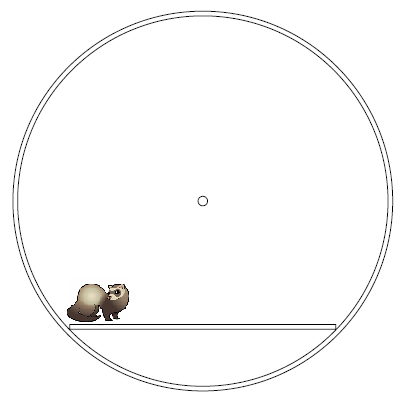
\includegraphics[width=0.35\textwidth]{ferret}
\end{center}
\caption{Ferret in a wheel.}
\label{fig:ferret}
\end{figure}

When the platform is released the ferret starts running, but, because of the ferret's motion, the platform and wheel remain stationary. Determine how the ferret moves.

\section*{Bonus}

Find out who dies in Fig. \ref{fig:whodies}.\\

\begin{figure}[h!]
\begin{center}
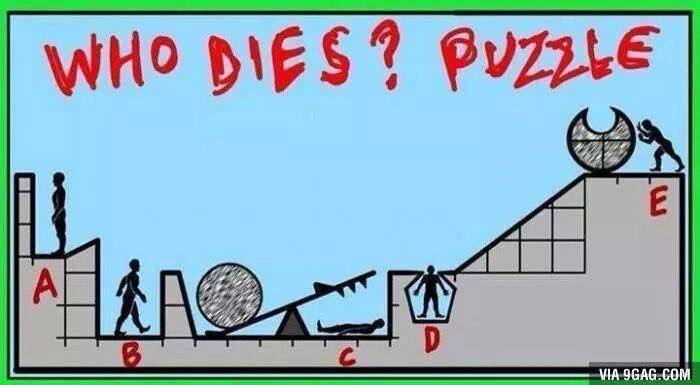
\includegraphics[width=1\textwidth]{whodies}
\end{center}
\caption{Who dies?.}
\label{fig:whodies}
\end{figure}

\end{document}